\documentclass[conference]{IEEEtran}
\usepackage{color}
\usepackage{booktabs} % For formal tables
\usepackage{multirow}
\usepackage{times}
\usepackage{flushend}
\usepackage{subfigure}
\usepackage{hyperref}
\usepackage{dsfont,amsfonts,amssymb,amsmath,color}
\usepackage{latexsym}
\usepackage{amsmath}
\usepackage{amsfonts}
\usepackage{algorithm}
\usepackage[noend]{algpseudocode}
\usepackage{graphicx}
\usepackage{bm}
\bibliographystyle{IEEEtran}

%\linespread{1.05} % Line spacing - Palatino needs more space between 
%\usepackage[utf8]{inputenc}
%\usepackage[T2A]{fontenc}
%\usepackage{float}
%\usepackage[left=2.5cm,right=2.5cm,asymmetric,top=32mm,columnsep=20pt]{geometry} % Document margins
%\usepackage[hang, small,labelfont=bf,up,textfont=it,up]{caption} % Custom captions under/above floats in tables or figures
%\usepackage{booktabs} % Horizontal rules in tables

%\usepackage{enumitem} % Customized lists
%\setlist[itemize]{noitemsep} % Make itemize lists more compact
\usepackage{float}
%\usepackage{abstract} % Allows abstract customization
%\renewcommand{\abstractnamefont}{\normalfont\bfseries} % Set the "Abstract" text to bold
%\renewcommand{\abstracttextfont}{\normalfont\small\itshape} % Set the abstract itself to small italic text
\usepackage{color,colortbl}

%\usepackage{titlesec} % Allows customization of titles
%\renewcommand\thesection{\Roman{section}} % Roman numerals for the sections
%\renewcommand\thesubsection{\textit{\Alph{subsection}}} % Alph numerals for subsections
%\titleformat{\section}{\large\scshape\centering}{\thesection.}{1em}{} % Change the look of the section titles
%\titleformat{\subsection}{\normalsize}{\thesubsection.}{1em}{\itshape} % Change the look of the section titles
\usepackage{graphicx}
%\usepackage{titling} % Customizing the title section

\usepackage{hyperref} % For hyperlinks in the PDF
\definecolor{lightRed}{RGB}{230,170,150}
\title{\LARGE \bf
Human motion analysis using Wi-Fi: A Review
}

\usepackage{graphicx}

% \author{ \parbox{3 in}{\centering Huibert Kwakernaak*
%         \thanks{*Use the $\backslash$thanks command to put information here}\\
%         Faculty of Electrical Engineering, Mathematics and Computer Science\\
%         University of Twente\\
%         7500 AE Enschede, The Netherlands\\
%         {\tt\small h.kwakernaak@autsubmit.com}}
%         \hspace*{ 0.5 in}
%         \parbox{3 in}{ \centering Pradeep Misra**
%         \thanks{**The footnote marks may be inserted manually}\\
%         Department of Electrical Engineering \\
%         Wright State University\\
%         Dayton, OH 45435, USA\\
%         {\tt\small pmisra@cs.wright.edu}}
% }

\author{ % <-this % stops a space
\thanks{}% <-this % stops a space
\thanks{$^{}$. 
        {\tt\small }}%
\thanks{$^{}$
        {\tt\small }}%
}

\begin{document}

\maketitle
\thispagestyle{empty}
\pagestyle{empty}


%%%%%%%%%%%%%%%%%%%%%%%%%%%%%%%%%%%%%%%%%%%%%%%%%%%%%%%%%%%%%%%%%%%%%%%%%%%%%%%%
\begin{abstract}
In this survey paper, we present a survey of recent advances in passive human activity recognition in indoor areas using the channel state information (CSI) of marketable Wi-Fi systems. We state some of the fundamental reasons why modern day researchers giving preference to CSI over traditional hardware based movement tracking systems. Different human body motions can causes alteration in the wireless motion images, as a result, variations in the CSI channel may occur. By assessing the data streams of CSIs for different activities and comparing them against stored models, human behavior can be recognized. This is done by separating features from CSI data streams and using machine learning techniques and algorithms to build prototypes and classifiers. Providing accurate and opportune information on people’s activities and behaviors is one of the most important tasks in pervasive computing. Innumerable applications can be visualized, for instance, in medical, security, entertainment, and tactical scenarios. Furthermore, this paper demonstrates variety of reasons that puts Wi-Fi’s CSI as more convenient method to evaluate human behavior compared to others. 


\end{abstract}


%%%%%%%%%%%%%%%%%%%%%%%%%%%%%%%%%%%%%%%%%%%%%%%%%%%%%%%%%%%%%%%%%%%%%%%%%%%%%%%%
\section{INTRODUCTION}

Recently, gesture recognition systems have become progressively interesting to researchers in the field of human computer interfaces. Specifically, the potential of device-free gesture recognition systems is the attraction that attracts researchers to this new and capable technology. Building interactive systems based on wireless signals (such as ubiquitous WiFi) that do not require installing cameras or sensors will eternally change the computing industry and smart device manufacturing: for example, when manufacturing a smart interactive TV, makers would not need to prepare the TV with expensive sensors or vision-based technologies; in its place, they could implement device-free gesture recognition technology. Therefore, this technology has the potential to deliver a tremendous innovation in the field of human computer interaction that can hugely affect both smart home systems, smart device manufacturing and health care services.
\newline
Human behavior recognition system plays a major role in
human-to-human interaction and interpersonal relationships.
Because it provides information about the identity of a
person, their facial shapes, and their personal activity. Where human behavior recognition could open up various fields of opportunities to advance human life, it also brings up many ways for an attacker to misuse such advance but easily handled technologies. Therefore, it is important to be aware of its misused if handled by a wrong hand.
\newline
The human ability to recognize another
persons’ activities is one of the main subjects of study of the
scientific area of artificial intelligence and machine learning
Applications such as Breathfinding: a wireless network that observers and localizes breathing in a home environment and detects the motion of human body that generates while breathing [2]. Similarly, Multi-person localization system has the ability to localize an user and track down his or her body movements solely through the reflections of wireless signals off his or her body, and functions just the same even if the user is the behind a wall or behind any sort of obstruction [3]. There are many more useful applications and techniques that have advanced human and machine learning developments and opened up several areas for researchers to improve them and design many of their security concerns. In previous human monitoring systems, the individual was to require to wear a device on the body set with tracking sensors such as gyroscope and accelerometer. The sensor data is managed locally on the wearable device or transmitted to a server in order to perform feature extraction; from there, controlled learning algorithms are used for categorization. \newline
As a result, opening up many opportunities for an outsider to manipulate this lengthy process and retain many personal data’s of the user.  This type of monitoring is known as active monitoring. For example, apple watches and Fitbit watches that are trendy to track human movements are considered as an active monitoring devices. Although such brand’s assures the security of personal data’s and interactions, there have been instances where these data’s were manipulated, causing several modifications of such devices before coming into humans’ everyday use. However, the performance of such system is shown to be around 90 percent for identification of activities such as sleeping, cooking, sitting, standing, walking, and running [4]. \newline
Nevertheless, always wearing a device is troublesome and may not be convenient for many impassive activity recognition applications, where the person may not be carrying any sensor or wireless device. While camera-built systems can be used for passive activity recognition, the line-of-sight necessity is a major limitation for such systems. Additionally, the camera-based methods have privacy issues and cannot be engaged in many locations that requires privacy. Therefore, a monitoring system that is solely based upon wireless signal, which does not violate the privacy of people, is desired. Because of common accessibility in indoor areas, lately, Wi-Fi has been the concentration of much research for activity recognition. Such systems consist of a Wi-Fi entry point and one or several Wi-Fi enabled devices situated at different areas of the environment. When a person participates in an activity, body positioning affects the wireless signals and alters the multi-path shape of the system. 
\newline
Rest of this paper is organized as follows: in section II, we discuss the application and some of the fundamental techniques of Wi-Fi method as well as how  CSI is used to extract the function of Wi-fi to apply to  determine human motion. In section III, we discuss several researches in this topic that extracts Wi-Fi's CSI to detect human motion. In section IV, we compare similar works that has been done in this topic and try to look at their similarities as well as the differences among these works. Section V demonstrates the methods and devices that are used to extract the Channel State Information (CSI) from a Wi-Fi signal. Section VI presents some of the recent research topics to strengthen and advance the field of Wi-Fi CSI to capture human motion.

\section{application of CSI (the core of WiFi technique)}
Channel State Information (CSI) of the wireless signals are accessible in many saleable devices. For example, CSI could be found in devices such as the Intel 5300 [2] and the Atheros 9390 system interface cards [3].  This information has a large range of functions and utilizations in many grounds like the use of CSI in the human activity recognition [4-8] (which is the main focus of this paper). CSI also expended in indoor localization [3,9],  human movement  of  falling  [4],  the  recognition  of  the existence of a human in a room or building [8] and even in the function of calculating the amount of people in a crowd [7]. Furthermore, other types of activity detection applications involve identifying the vocalized words by using a dedicated directional antenna to obtain the necessary CSI variations caused by movements of the lips during speaking [5]. \newline
CSI can also be used to recognize daily human life activities using the E-eye system as example [6]. Wikey  [10],  Wi-Vi  [11],  WiHear  [5],  and WiDraw [13] are all just other examples of the versatile applications that can make use  of the CSI. [5]
The three-dimensional qualities of radiated wireless signals are the source of location distinction and purpose for wire-less indoor localization. Available in mainstream wireless signal measurements, the Received Signal Strength Indicator (RSSI) has been adopted in vast indoor localization systems. The following graph shows such passive radar methods.

\begin{figure}[h!]
    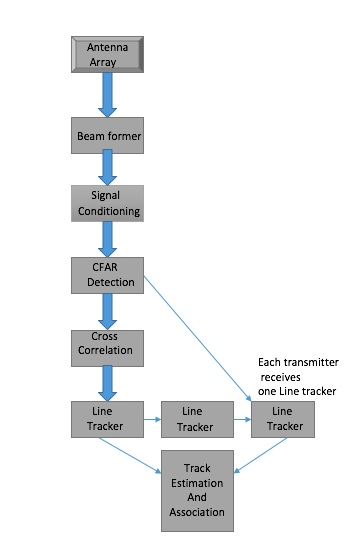
\includegraphics[scale=0.45]{Figure11.png}
    \caption{Antenna tracker}
    \label{fig:me}
\end{figure}

However, it suffers from dramatic performance
degradation in complex situations due to multipath fading
and temporal dynamics [7]. Recently, researchers have tried
to leverage wireless physical layer channel state information
(CSI) in place of wireless medium access layer received
signal strength indicator (RSSI), since CSI achieves finer
sensing granularity and can use information dimensions
to obtain a qualitative improvement. Unlike RSSI, CSI is
measured from radio links per 
OFDM subcarriers of each received packet.
Therefore, CSI has more information since RSSI value is
only per received packet. Moreover, CSI is more robust to
complex environments. As a result, CSI helps in building a
more sophisticated, more sensitive, and more robust sensing model. Such progress also makes more sophisticated sensing
applications become more possible. Accordingly, in recent
years CSI has been leveraged in different device-free such
as human localization, motion detection, activity recognition
and gesture recognition.

% table started
\begin{table}[h]
\caption{References of hardware's to collect Wi-Fi Signal}
\label{table_example}
\begin{center}
\begin{tabular}{|c||c|}
\hline
        References & Radar/Hardware  \\
\hline
Fadel Adib et. al. [8] & FMCW Radar \\
\hline
\hline
Qifan Pu et.al. [5] & Through the wall radar system \\
\hline
\hline
Fadel Adib et. al. [35] & Inverse synthetic aperture radar (ISAR) \\
\hline
Guanhua Wang [6] & Doppler Shift Radar ISAR \\
\hline
D. Huang [19] & Imaging radar \\
\hline
Z. Kabelac [23] & FMCW Radar \\
\hline
Neal Patwari [2] & Doppler shift \\
\hline
Martina Broetje [36] & Passive Radar \\
\hline
Fadel Adib [37] & Doppler Radar, Ultrawithband Radar, FMCW \\
\hline
Mingmin Zhao [38] & FMCW \\
\hline
Fadel Adib [3] & FMCW, imaging radar \\
\hline
\end{tabular}
\end{center}
\end{table}
% Table ended

\section{Related Works}
Human motion recognition has increasingly attracted intense academic and industrial interest due to its many applications in real life such as health care, fitness tracking etc [1]. In general, traditional human tracking system have been considered a device based approaches such as vision based, body worn sensor etc. However, both vision based camera and body worn sensors has certain limitations. To explain, vision based sensors cannot be used under a dark area or low light environment. Also, body worn sensor cannot be wore everywhere or all the time, such as it cannot be used in the bathroom or while taking shower. Moreover, they invade human privacy. In recent researches, Wi-Fi signal built human gesture recognition devices, such as Wisee[5], Wi-sleep [6], Breathfinding, have been proposed based on the observation that different human activities introduce different multi-path distortions in Wi-Fi signals. 
\newline
Although device-free systems do not need a person to hold or carry any devices, it need a dense placement of sensors to make a mesh of wireless links within region of interest. The uses of specified physical layer measures such as Doppler shifts from one single wireless identify people’s motion movement, position, even their actions which involves the roughness ranges from coarser activities to fine-grained gestures (such as Wisee [5] and Wi-Track[8]). Nevertheless, these applications all are outlined to use USRP software radio and require a specified receiver that extricates wave features that are not described in current Wi-Fi systems, encouraging researchers toward using CSI, which can be very easily accessed from today’s commodity devices and processed by the improved driver. Table 1 highlights the uses of distinct radars and hardware’s that was used by many recent researches using Wi-Fi network to detect human gestures. With CSI, more movements and even human actions are magnificently recognized, giving growth to many interesting research topics and their applications. \newline
For example, E-eyes [9] presents a user-feedback system, separating actions into walking and in-place activity, that is capable of distinguishing many paths and activities. WiHear [6] processes CSI for mouth motion profiles in order to understand the way people talk and comprehend what people say. CARM [10] introduces a de-noising method built on principal component analysis (PCA) followed by discrete wavelet transform (DWT), and provisions human activity recognition independent of environment variances. Nonetheless, parts of the features used in CARM [10] are related to the time duration of an action, which to our knowledge, might render classifiers highly vulnerable to duration estimation errors. Also, despite the promising results, most works involve domain knowledge specifically related to the defined scenarios such as WiFall [11] primarily designed for fall detection. Because of its high sensitivity to environmental differences caused by moving objects, researchers start studying the possibility of Wi-Fi identification. \newline


\begin{figure}[h!]
    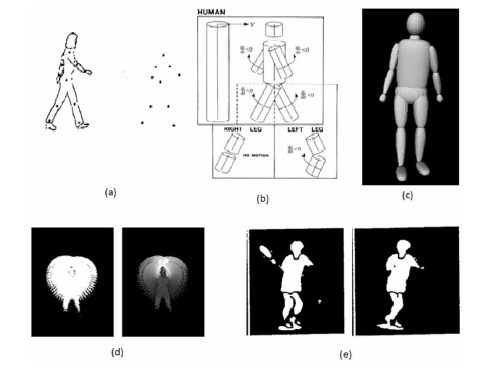
\includegraphics[scale=0.40]{fig7.png}
    \caption{Wi-Fi CSI is being captured in human motion}
    \label{fig:me}
\end{figure}





In FreeSense [12], Tong et al. propose a method that recognizes the line-of sight path crossing instants followed by PCA and DWT to extract features and achieve an accuracy of 90 percent in a six-person scenario. However, their method would work only if a subject pass across the LOS path. WifiU [13] also connects PCA to lessen the uncorrelated noises in distinctive subcarriers. By applying short-time Fourier transform to convert PCA modules into spectrograms, it attains a top-1 accuracy of 92 percent. However, several of their features such as walking pace, gait cycle time, would be unsuccessful when applied on some actions that does not include walking. For instance, actions such as jump do not implicate movement speed or period. \newline
Furthermore, CSI from profitable APs, some researchers apply directional antennas or antenna array to extract more complete information, reaching a better localization resolution and understanding more powerful applications. For example, RFCapture [14] designs an unique device using a T-shape antenna array and Frequency Modulated Carrier Wave (FMCW) to recognize human movements through wall. The antenna array distinguishes the route of gestures and the frequency cheap calculates the delay of received signals by repetitively adjusting the transmitted signals. Likewise, WiTrack [8] uses a similar device to identify a person in 3D space through wall. All of these recent works that have been mentioned requires modest commercial APs with only Omni-directional antennas, which are affordable and universal.

\begin{figure}[h!]
    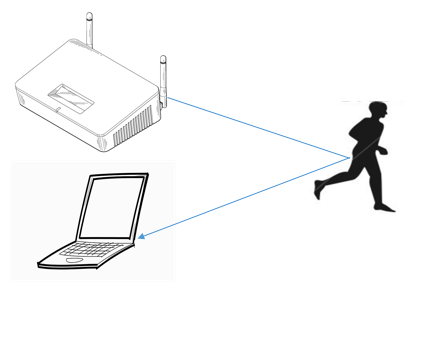
\includegraphics[scale=0.45]{fig16.png}
    \caption{A simple process to capture human motion by recent human motion detection devices}
    \label{fig:me}
\end{figure}

\section{Comparative Studies}
Present work on device-free human activity identification can be separated into four major categories: Received Signal Strength Indicator (RSSI) based, specialized hardware based, radar based, and CSI based. Below are the breakdown of uses of these particular infrastructures in recent researches. 
\subsection{RSSI Based}
RSSI based human activity recognition techniques influence the signal strength changes caused by human activities [15,16, 17]. This tactic can only do coarse grained human activity recognition with low exactness because the RSSI values provided by the commercial devices consist very low resolution [17]. For RSSI based gesture recognition, the accuracy is 56 percent over 7 distinctive gestures [15]. Some devices use software radio to increase the granularity of RSSI values and therefore expand the accuracy of activity recognition to 72 percent for 4 activities [16]. 
\begin{table}[h]\caption{\label{tab:statistic}Comparison of the used hardware's}\small\vspace{-0.1in}
\centering 
\begin{tabular}{cccc}
\toprule
Work & Software-defined & Antenna & Frequency-Wave \\
WiSee[9] &  Yes &  Yes &   Yes \\
AllSee[10] & Yes & Yes & No \\
E-eyes[15] & No & Yes & Yes \\
CARM[17] & No & Yes & Yes \\
RF-Capture & Yes & Yes & No \\
Wi-Track & No & Yes & Yes \\
\bottomrule
\end{tabular}
\end{table}
\subsection{ Specialized Hardware Based }
 Fine-grained radio signal measurements can be collected by software defined radio or specially designed hardware [11, 12, 14, 17]. WiSee uses USRP to capture the WiFi OFDM signals and measures the Doppler shift in signals returned by human bodies to identify a set of nine distinctive movements with an accuracy of 95 percent [17]. AllSee uses a specifically designed analog circuit to extract the amplitude of the received signals and uses their envelopes to distinguish motions within a short distance of 2.5 feet [14]. Wision uses multi-path reflections to create an image for adjacent objects [11].
 \subsection{ Radar Based }
 Device-free human motion identification system has also been learned using radar technology [4, 5, 16, 25]. Through the micro Doppler information, radars can measure the movement speeds of different parts of human body [25]. WiTrack uses specially designed Frequency Modulated Carrier Wave (FMCW) signals to track human movements behind the wall with a resolution of approximately 20cm [4, 5]. Compared to the particularly designed radar signals such as FMCW or Ultra-wideband (UWB) signals, WiFi signals have far narrower bandwidth. For example, 802.11a/b/g usually use a bandwidth of 20 MHz, while FMCW uses bandwidth of up to 1.79 GHz [4]. 
 \subsection{CSI Based}
CSI standards are accessible in many commercial devices such as Intel 5300 [9] and Atheros 9390 network interface cards (NICs) [19]. Lately CSI has been used for human activity recognition [1,2,3,4,5,6,12,14,15,16,20,25] as well as indoor localization [19,32]. Han et al. offered to use CSI to detect a single human activity of falling [10]. Zhou et al. proposed to use CSI to detect the existence of a person in an location [35]. Xi et al. proposed to use CSI to calculate the number of people in a crowd [30]. WiHear uses expert directional antennas to find CSI distinctions caused by lip movement for identifying spoken words [26]. E-eyes identifies a set of nine daily human activities using CSI. WiHear and E-eyes use CSI in rather different means than CARM. WiHear does not effectively denoise CSI values; thus, it has to use directional antennas to ease the noise in CSI values to attain adequate exactness. In contrast, CSI values uses commercial WiFi devices with built-in omni directional antennas. E-eyes uses CSI histograms as fingerprints for identifying human everyday actions, such as brushing teeth, taking showers, and washing dishes, which are moderately location reliant.
\newline
Moreover, E-eyes uses Channel State Information (CSI) histograms as fingerprints for recognizing daily human activities. Similarly, Wi-hear uses a specialized directional antenna to obtain CSI variations cause by one’s lip movements for recognizing spoken words. Wi-see uses USRP to capture the OFDM signals and measures the Doppler shift in signals reflected by human bodies to recognize up to nine human gestures. The major advantages of such inventions over camera based or sensor based approaches is that they can operate through walls, low light sightings. Although such devices dot not raise much of security issues, CSIsnoop shows that an attacker holds the ability to even infer CSI in a multi-user WLAN, even when both channel signaling sequences from the access point and CSI measurement pointer from the clients are encrypted [25]. 


\section{WIFI CSI SIGNAL PROCESSING AND BEHAVIOR RECOGNITION METHODS}
Signal processing and machine learning both methods are used in combination with Wi-FI CSI dimensions for human behavior recognition and movement monitoring. In this section of the paper, we will demonstrate numerous tactics which have been used to extract Wi-Fi CSI, which will be including those that have been used to recognize frequency (Doppler) shifts produced from bodily movements in the area of a Wi-Fi AP. We also examine the approaches used to categorize CSI/Doppler innate to a given motion, and the possible enhancements afforded by making use of sequential patterns within the frequency data. Figure 2 illustrates the main processing and classification steps in scenarios where people move through Wi-Fi fields.

\begin{figure}[h!]
    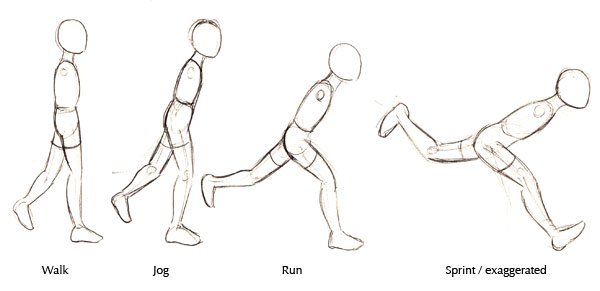
\includegraphics[scale=0.35]{fig12.png}
    \caption{Scenarios where people move through a Wi-Fi field}
    \label{fig:me}
\end{figure}

\subsection{ Extracting the WiFi CSI }
Commercial Off-the-Shelf Devices: The mainstream of commercial WiFi-enabled devices is able to parse WiFi signal data and output report about the state of the channel, the most conjoint being the received signal strength indicator (RSSI). Nevertheless, factors such as the location of disperses, multipath and shadowing act as main causes of error in RSSI measurements. Procedures such as ’Fingerprinting therefore need initial description actions within an setting, prior to carrying out any localization tasks. More lately, researchers have taken benefit of the Intel 5300NIC to capture WiFi CSI. It uses pilot OFDM symbols in 802.11n signal to approximate the CSI, and reports the channel matrices for 30 subcarrier groups from 3 accepting antennas. Each matrix holds compound accesses with signed 8-bit resolution each for both the real and imaginary parts. The restrained phase on each receipt antenna provides a chance to use well-established signal managing methods, a popular method being the subspace based joint angle and time approximation system on the basis of Schmidt Orthogonalization [13]. Fig 3 demonstrates a cycle of human movements and the process of CSI to capture that movement.
\newline

\begin{figure}[h!]
    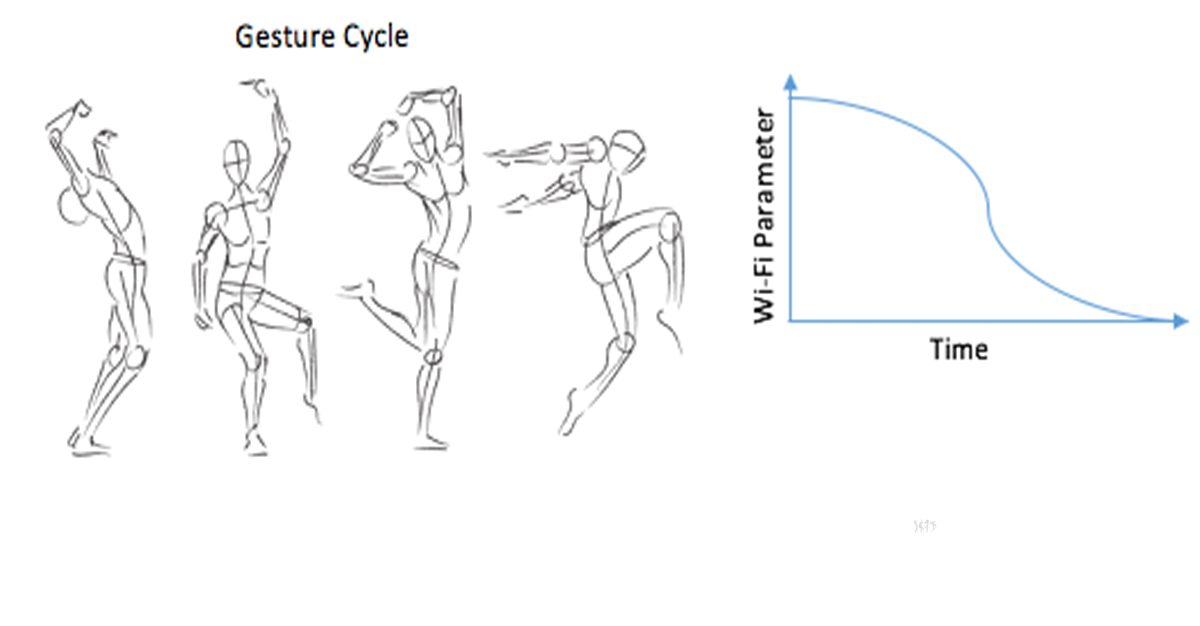
\includegraphics[scale=0.20]{fig4.png}
    \caption{A cycle of human gestures that captured by home Wi-Fi}
    \label{fig:me}
\end{figure}


Dedicated Devices: Software defined radio (SDR) systems have normally been used to gain raw WiFi data in order to apply altered signal handling for extracting CSI. For example, xDtrack [3] applies a subspace search method on raw IQ samples to resolve phase differences for high-resolution ToA and AoA approximations. By taking additional IQ samples, passive WiFi sensing [9] is able to determine channel Doppler shifts at very high resolution as well. The signal processing method in [9] retains the cross ambiguity function (CAF) to compare the original WiFi transmission with deliberate reflections to classify small Doppler shifts ensuing from moving people. Especially for Doppler shift and frequency component, there are two main methods. One approach is to apply STFT or DWT on CSI for obtaining frequency component. Nevertheless, this approach has a restriction on distinguishing moving object reflections and stationary reflections. Another tactic which is built on passive radar principle applies CAF managing on experimented signals from reference and surveillance channels that holds stationary source signal and moving object reflection correspondingly. The reflexive radar approach shows good performance on abandoning the impact from stationary reflection. The following image shows the CSI data collection process:
\begin{figure}[h!]
    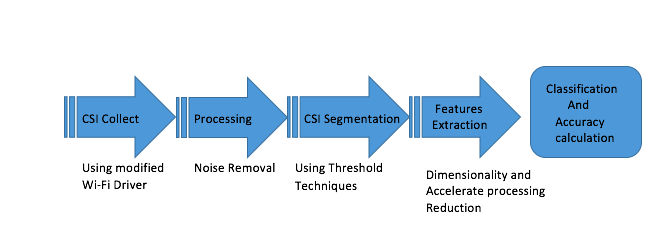
\includegraphics[scale=0.35]{fig10.png}
    \caption{CSI data collection Process}
    \label{fig:me}
\end{figure}



\subsection{Behavior Recognition}
Temporal Channel State Differences: At any particular instant, a measurement of the WiFi channel state provides tiny information relating to the behavior of a person in the signal broadcast path. However, evaluating the CSI as an instance of time offers this possibility: a physical change in a person’s location, speed and/or path will affect propagation paths, Doppler shifts and advent angles. The effect is an alteration in the channel with a distinguishing temporal signature. Even if a person tries to stand still, the movement of their chest will give rise to time unreliable proportionate changes in the phase, frequency and amplitude features of the reflected signal. In practice, an usual gesture cycle such as that shown in Figure 2 will be made up of a mixture of gestures from various parts of the body, leading to a compound temporal signature. We find that certain CSI structures actually demonstrates a clear change in their chronological trace during one wave cycle when there is one primary motion and minimum intrusion and noise - see Figure 2 (b). However, as illustrated in Figure below, when there are multiple contributory motions during a gesture cycle, CSI parameters change in a more complex manner. 

\begin{figure}[h!]
    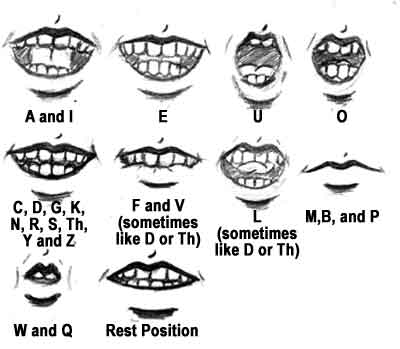
\includegraphics[scale=0.40]{fig13.png}
    \caption{Human lip movements that can be captured Wi-Fi [20]}
    \label{fig:me}
\end{figure}

\subsection{Feature Extraction}
The performance of a classifier for recognizing activities and behaviors depend vastly on correctly forming and extracting various characteristics in a a gesture cycle measurement. As can be seen from Figure 6, some CSI limitations show a familiar pattern during the gesture period. While it is difficult to extract intuitive features in a general case, matrix analysis can be applied to study structural properties during a gesture period, and usual approaches include Principle Component Analysis (PCA) and the Singular Value Decomposition (SVD). 
\subsection{Classification of Gestures/Activities}
A wide range of health care monitoring uses require real-time ordering of a movement or activity, for example falling down, so that a warning can be instantaneously activated. Many of the classifiers are capable to meet this condition but their applicability also relies on the kind of input features selected. Overall, the most popular classification systems are the Naive Bayesian classifier, support vector machine (SVM) classifier and the sparse representation classifier (SRC). The Naive Bayesian classifier is naive and flexible to feature types but only appropriate for little number of features. 



\section{Recent research topics on wifi utilization}
Human Computer Interaction (HCI) is growing very fast in our everyday life needs. In section of the paper, we will examine some common researches that have been done on this area that has the huge potential to open many more research areas on this field. We know that  the old solutions to control computing devices and smart applications in the smart environments includes using cameras [14] that track human 
movements and try to classify and recognize these movements by comparing the collected data to an already kept patterns. The other traditional way of recognizing human activities included Radar [15] or wearable devices (like sensors or smart watches) [16, 17]. As we already know, in many area camera based methods have the several limitations of requiring line of sight (LoS) with enough lighting and the potential privacy breaching of humans. 
\newline 
However, the recent device-free location-oriented activity identification at home using the existing WiFi Access Points (AP) and the WiFi devices such as, desktops, thermostats, smart TVs, laptops etc which comes with low cost as a result. To elaborate, in E-eyes, the low-cost system takes benefit of the profusion of WiFi links between such devices and the increasingly fine-grained CSI that could to be extracted from such links. It examines channel features and can uniquely identify both in-place activities and walking movements across a home by comparing 
them against signal profiles. Signal profiles construction can be semi-supervised and the 
profiles can be adaptively updated to accommodate the movement of the mobile devices and day-to-day signal calibration. E-eyes systems idea includes using the existing 
channel state information (CSI) provided by IEEE 802.11n devices and relatively few 
wireless links, such as those to existing in-home WiFi devices as shown in the figure 7:

\begin{figure}[h!]
    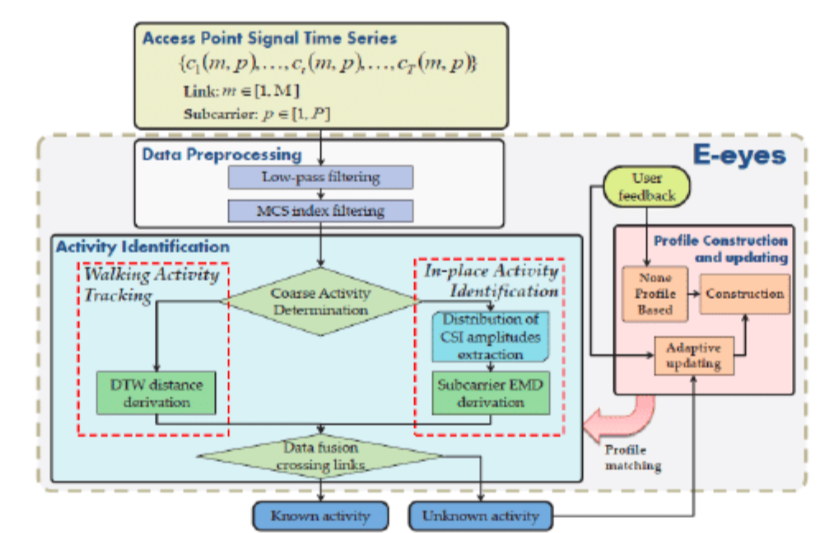
\includegraphics[scale=0.30]{fig2.png}
    \caption{E-eyes capturing human motion [26]}
    \label{fig:me}
\end{figure}


Another form of applications of the wireless signals information include seeing through the 
walls and one example of it is the Wi-Vi [11]. This system is a wireless device that captures 
moving objects behind a wall. It controls the ubiquity of WiFi to make through wall 
imaging relatively very low-cost, low-bandwidth, and usable and affordable to average users
Wi-Vi uses WiFi OFDM motions in the ISM band (at 2.4 GHz) and makes use of WiFi 
hardware. Wi-Vi is basically a 3-antenna MIMO device: two of the antennas are used for 
transmitting and one is used for receiving. It also uses directional antennas to focus toward the wall or the area of interest. Its design includes two key components: 
1) The first section removes the flash reflected off the wall by performing MIMO 
nulling. 2) The second part tracks a moving object by handling the object itself as an antenna array exhausting a method called Inverse Synthetic Aperture Radar (ISAR). \newline
Moreoever, the Wi-Vi system can be expended in one of two distinct modes, varying on the user’s choice. To explain, in mode 1, it can be used to capture any sort of moving objects behind a wall and track them. In mode 2, instead, Wi-Vi functions as a signal based interface from behind a wall that allows humans to compile messages and send them to the Wi-Vi receiver. The other example of such system is the system 
suggested in [12] that is also pointing to see behind the objects and behind walls but this system required both the transmitter and a receiver to be contained inside of the subjected room in order to process. \newline
Furthermore, using CSI, some recent research efforts have been focusing of answering the question if Wi-Fi could be used to hear human voices and the system in [5] WiHear, discovers the probable of using WiFi to hear  people talk and transmit  the  talking information to the sensor at the same time. 
WiHear introduces a new way to hear people talks without the need of using any aural sensors. Furthermore, it  still works  well even when the surrounding setting is noisy. As a result
 WiHear will bring a new interactive interface between human and devices, which allows devices to sense and recognize more complex human behaviors with negligible cost. In practical life, WiHear can help millions of disabled people to handle simple commands to devices with only mouth signs instead of dense and inconvenient body movements.  WiHear first locates the mouth of an individual, and then reads the words by monitoring the signal reflections from one’s mouth.  As it recognizes mouth moving shapes, WiHear can obtain talking information the similar way as lip reading.  Thus, WiHear presents a micro-motion detection structure  that  can  differentiate among different mouth movements with different letters as shown in figure 6 [5]. WiHear frame includes  filtering,  partial multipath  removal,  wavelet  transform, segmentation,  feature  extraction,  and  finally classification and error correction.
 
 \begin{figure}[h!]
    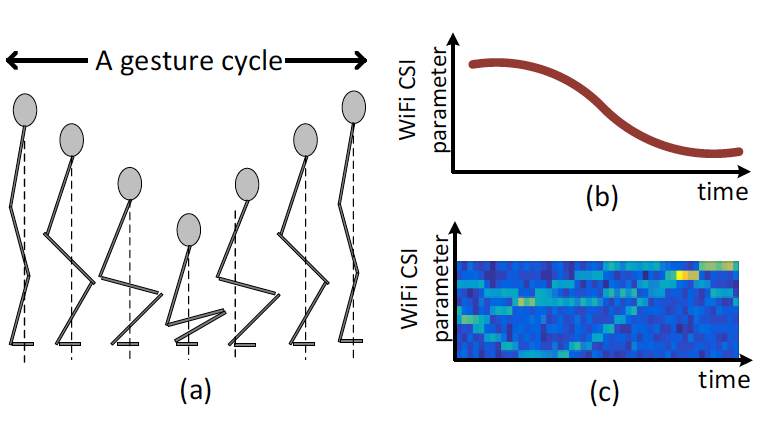
\includegraphics[scale=0.35]{fig6.png}
    \caption{Wi-Fi CSI in used to capture human gesture cycle}
    \label{fig:me}
\end{figure}


\section{Current researches in CSI}
An attacker can deduce CSI in a multi-user WLAN, even if both channel sounding sequences from the point of the access and CSI dimension pointer from the clients are encrypted. CSI of clients can be computed based on transmit beamforming weights at the access point, and that the transmit beamforming weights can be estimated from downlink multi-user transmission [20]. For example, CSIsnoop, a software that organize experiments in many indoor areas and the results show that on average CSIsnoop can deduce CSI of the target user with a total standardized connection, thereby pressing reevaluation of the use of CSI as a tool to improve substantial layer security in multi-user WLANs.
Channel State Information (CSI) plays a huge role in multi-user beamforming systems as it allows an Access Point (AP) to increase data by simultaneously sending several data streams to multiple users. \newline
According to IEEE 802.11ac/af [7, 8], an identified channel sounding sequence is transmitted by the AP, and from where a user compute and feedback their measurement results of the channel’s outcome on the known system. Built on the gathered CSI, the AP can compute transmit beamforming powers and, for example, zero-force the signals of one user at other users in order to eliminate inter-user interference [25]. Moreover, CSI can be also used to increase network throughput by grouping user with orthogonal channels [25]. Besides data transmission, CSI has also been proposed to enhance network security as it decorrelates over half a wavelength in many environments and enhance quality. 
\newline
Hence, wireless devices can retain CSI in order to establish a secret key[12], which seems especially auspicious when there are a very few resources or lacking key management substructure. Finally, CSI can be useful to add artificial noise orthogonal to the proposed recipient to degrade a spy's channel [1, 5]. This kind of artificial noise is nulled at the clients by the AP so that the signal SINR at the clients will not be reduced. Because of the importance of CSI, it has been proposed to encrypt CSI during the standard-defined explicit channel sounding process: either by encrypting the measurement feedback from the users, or by encrypting the channel sounding sequence from the AP [19]. Therefore, a node within array of the network cannot learn clients’ CSI by hearing their measurement feedback [20]. \newline
However, several recent researches shows that the above method cannot generate accurate privacy methods. For example, CSIsnoop presents a structure by which a passive attacker can deduce the CSI of clients by recognizing their downlink beamforming communication. To proceed, CSIsnoop would retain the information of part of the transmitted marks and trains an adaptive filter to distinct the different data servers at the multiple-antenna malicious node (Eve), The malicious node subsequently estimates the channel from the AP and combines it with the adaptive filter to compute the transmit beamforming weights that the AP must have used. Finally, it uses the probable beamforming weights to figure the CSI of clients. 


\section{Conclusion}
In this work, a survey of recent researches in human activity recognition systems using WiFi CSI system has been introduced. The importance in this area shows great promise in achieving good accuracy in indoor environments. Using numerical test, it has been observed that better accuracy can be obtained by employing deep learning techniques. There are still many challenges that need to be worked on by future researchers such as, how to make the system more robust in different broader and dynamic environments, how to use the advantage of CSI in more open outdoor areas, and how to identify the behaviors of multiple users as well as considering several security points.


\begin{thebibliography}{99}

\bibitem{c1} “Michalis Vrigkas, Christophoros Nikou and Ioannis A. Kakadiaris: A review of human activity recognition methods. In Proceding’s of ACM Mom, 2015”

\bibitem{c2}“Neal Patwari, Lara Brewer, Quinn Tate, Ossi Kaltiokallio: Breathfinding: A wireless network that monitors and locates breathing in a home. In Proceedings of ACM MobiCom, 2014”

\bibitem{c3} “Fadel Adib Zachary Kabelac Dina Katabi:
 Multi-user localization via RF body reflections. In Proceedings of IEEE INFOCOM, 2015”

\bibitem{c4} “Heba Abdelnasser, Moustafa Youssef, Khaled A. Harras: Wi-Fi-based real time calibration – free passive human motion detection. In Proceedings of Usenix NSDI, 2014. ”

\bibitem{c5}“Qifan Pu, Siyu Jiang, and Shyamnath Gollakota: Wi-see: Whole home gesture recognition using wireless signal. In Proceeding of ACM MobiSys, 2013 ”

\bibitem{c6} “Guanhua Wang, Yongpan Zou, Zimu Zhou, Kaishun Wu: Wi-hear: We can hear you with W-Fi, In Proceedings of IEEE INFOCOM, 2014”

\bibitem{c7} “Zheng Yang, Zimu Zhou, Yunhao Liu: From RSSI to CSI: Indoor Localization via Channel Response, 2013”

\bibitem{c8}“Fdel Adib, Zachary Kabelac, Dina Katabi: Wi-track: 3d tracking via body radio reflections, 2015. In Proceedings of IEEE INFOCOM, 2013”

\bibitem{c9}“Wei Wang, Alex X. Liu, Muhammad Shahzad: Understanding and Modeling of WiFi Signal Based Human Activity Recognition

\bibitem{c10} “Chunmei Han, Kaishun Wu, Yuxi Wang: Wi-fall: WiFall: Device-free Fall Detection by Wireless Network. In Proceedings of ACM MoMM, 2013 ”

\bibitem{c11} “Jin Zhang, Bo Wei, Wen Hu: WiFi-ID: Human Identification using WiFi signal, 2014”

\bibitem{c12} “Chenshu Wu, Zheng Yang, , Zimu Zhou: Non-Invasive Detection of Moving and Stationary Human With WiFi, 2015”

\bibitem{c13} “Fadel Adib Chen-Yu Hsu Hongzi Mao: Capturing the Human Figure Through a Wall”

\bibitem{c14} “H. Abdelnasser, M. Youssef, and K. A. Harras. WiGest: A ubiquitous wifi-based gesture recognition system. In Proceedings of IEEE INFOCOM, 2015.”

\bibitem{c15}] “S. Sigg, M. Scholz, S. Shi, Y. Ji, and M. Beigl. RF-sensing of activities from non-cooperative subjects in device-free recognition systems using ambient and local signals. IEEE Transactions on Mobile Computing, 13(4):907–920, 2014.”

\bibitem{c16} “S. Sigg, S. Shi, F. Buesching, Y. Ji, and L. Wolf. Leveraging RF-channel fluctuation for activity recognition: Active and passive systems, continuous and rssi-based signal features. In Proceedings of ACM MoMM, 2013.”

\bibitem{c17} “Zhang, Xu, W. Knightly, Edward. CSIsnoop: Attacker Inference of Channel State Information in Multi-User WLANs. 1-10. 10.1145/3084041.3084048.”


\bibitem{c18} S. Sigg, U. Blanke, and G. Troster. The telepathic phone: Frictionless activity recognition from WiFi-RSSI. In IEEE PerCom, pages 148–155, 2014.”

\bibitem{c19} “D. Huang, R. Nandakumar, and S. Gollakota. Feasibility and limits of Wi-Fi imaging. In Proceedings of ACM SenSys, pages 266–279, 2014. ”

\bibitem{c20} “B. Kellogg, V. Talla, and S. Gollakota. Bringing gesture recognition to all devices. In Proceedings of Usenix NSDI, 2014.”
\bibitem{c21}“B. Lyonnet, C. Ioana, and M. G. Amin. Human gait classification using microdoppler time-frequency signal representations. In Proceedings of IEEE Radar Conference, pages 915–919, 2010.”
\bibitem{c22} “G. Wang, Y. Zou, Z. Zhou, K. Wu, and L. M. Ni. We can hear you with Wi-Fi! In Proceedings of ACM MobiCom, 2014.”
\bibitem{c23} “Z. Yang, Z. Zhou, and Y. Liu. From RSSI to CSI: Indoor localization via channel response. ACM Computing Surveys, 46(2):25, 2013.”

\bibitem{c24} “Z. Zhou, Z. Yang, C. Wu, L. Shangguan, and Y. Liu. Towards omnidirectional passive human detection. In Proceedings of IEEE INFOCOM, pages 3057–3065, 2013.”

\bibitem{c25} “Zhang, Xu, W. Knightly, Edward. CSIsnoop: Attacker Inference of Channel State Information in Multi-User WLANs.”

\bibitem{c26} “Yan Wang, Jian Liu and Yingying Chen, Marco Gruteser, Jie Yang, Hongbo Liu. E-eyes: device-free location-oriented activity identification using fine-grained WiFi signatures. MobiCom 2014.”



\end{thebibliography}

\end{document}
